\section{Fourier Series}

\subsection{Periodic Functions}
\begin{definition}[Periodic function]
    A function $f(x)$ is \vocab{periodic} if $f(x+T) = f(x)$ for all $x$, where $T$ is the \textit{period}.
\end{definition} 
For example, simple harmonic motion is periodic.
In space, we consider the wavelength $\lambda = \frac{2\pi}{k}$, and the (angular) wave number $k$ is defined conversely by $k = \frac{2\pi}{\lambda}$.

% \subsection{Properties of trigonometric functions}
Consider the set of functions
\begin{align*}
    g_n(x) = \cos \frac{n\pi x}{L};\quad h_n(x) = \sin \frac{n\pi x}{L}
\end{align*}
where $n \in \mathbb N$.
These functions are periodic on the interval $0 \leq x < 2L$ with period $T = 2L$.
Recall that
\begin{align*}
    \cos A \cos B & = \frac{1}{2}\qty(\cos(A-B) + \cos(A+B)); \\
    \sin A \sin B & = \frac{1}{2}\qty(\cos(A-B) - \cos(A+B)); \\
    \sin A \cos B & = \frac{1}{2}\qty(\sin(A-B) + \sin(A+B))
\end{align*}

% \subsection{Periodic function space}
\begin{definition}[Inner product]
    We define the \vocab{inner product} for two periodic functions $f, g$ on the interval $0 \leq x < 2L$.
    \begin{align*}
        \inner{f, g} = \int_0^{2L} f(x) g(x) \dd{x}\footnote{We will generalise this definition later when we use other eigen functions.}
    \end{align*}
\end{definition} 

The functions $g_n$ and $h_n$ are \textit{mutually orthogonal} on the interval $[0, 2L)$ with respect to the inner product above.
\begin{align*}
    \inner{h_n, h_m} & = \int_0^{2L} \sin \frac{n\pi x}{L} \sin \frac{m\pi x}{L} \dd{x} \\
    & = \frac{1}{2} \int_0^{2L} \qty(\cos\frac{(n-m)\pi x}{L} - \cos \frac{(n+m)\pi x}{L}) \dd{x} \\
    & = \frac{1}{2} \frac{L}{\pi} \qty[ \frac{1}{n-m}\sin\frac{(n-m)\pi x}{L} - \frac{1}{n+m} \sin \frac{(n+m)\pi x}{L} ]_0^{2L} \\
    & = 0 \text{ when } n \neq m
\end{align*}
If $n = m$, we have
\begin{align*}
    \inner{h_n, h_n} = \int_0^{2L} \sin^2 \frac{n\pi x}{L} \dd{x} = \frac{1}{2} \int_0^{2L} \qty(1-\cos \frac{2\pi n x}{L}) \dd{x} = L \quad (n \neq 0)
\end{align*}
Thus,
\begin{align} \label{eq:1.1}
    \inner{h_n, h_m} = \begin{cases}
        L \delta_{nm} & n,m \neq 0 \\
        0             & nm = 0
    \end{cases}
\end{align}
Similarly, we can show
\begin{align} \label{eq:1.2}
    \inner{g_n, g_m} = \begin{cases}
        L \delta_{nm} & n,m \neq 0                                 \\
        0             & \text{exactly one of } m,n \text{ is zero} \\
        2L            & n,m = 0
    \end{cases}
\end{align}
and
\begin{align} \label{eq:1.3}
    \inner{h_n, g_m} = 0
\end{align}
Now, we assert that $\qty{g_n, h_n}$ form a complete orthogonal set; they span the space of all `well-behaved' periodic functions of period $2L$.
Further, the set $\qty{g_n, h_n}$ is linearly independent.

\subsection{Definition of Fourier series}
Since $g_n, h_n$ span the space of `well-behaved' periodic functions of period $2L$, we can express any such function as a sum of such eigenfunctions.
\begin{definition}[Fourier series]
    The \vocab{Fourier series} (FS) of $f$ is
    \begin{align} \label{eq:1.4}
        f(x) = \frac{1}{2}a_0 + \sum_{n=1}^\infty a_n \cos \frac{n \pi x}{L} + \sum_{n=1}^\infty b_n \sin \frac{n \pi x}{L}
    \end{align}
    where $a_n, b_n$ are constants such that the right hand side is convergent for all $x$ where $f$ is continuous.\footnote{Note does not require differentiability unlike a Taylor series.}
\end{definition}
At a discontinuity $x$, the Fourier series approaches the midpoint of the supremum and infimum of the function in a close neighbourhood of $x$.
That is, we replace the left hand side with
\begin{align*}
    \frac{1}{2}f(x_+) + \frac{1}{2}f(x_-)
\end{align*}

Let $m > 0$, and consider taking the inner product $\inner{h_m, f}$ and substituting the Fourier series of $f$.
\begin{align*}
    \inner{h_m, f} &= \int_0^{2L} \sin\frac{m \pi x}{L} f(x) \dd{x} \\
    &= \int_0^{2L} \sin\frac{m \pi x}{L} \left( \frac{1}{2}a_0 + \sum_{n=1}^\infty a_n \cos \frac{n \pi x}{L} + \sum_{n=1}^\infty b_n \sin \frac{n \pi x}{L} \right) \dd{x} \text{ by substituting \cref{eq:1.4}}\\
    & = \inner{h_m, b_m h_m} \text{ by orthogonality relations \cref{eq:1.1,eq:1.2,eq:1.3}}\\
    & = L b_m
\end{align*}
Thus,
\begin{equation}
    \begin{aligned}
    b_n = \frac{1}{L} \inner{h_n, f} = \frac{1}{L} \int_0^{2L} \sin\frac{n \pi x}{L} f(x) \dd{x} \\
    % \intertext{and analogously}
    a_n = \frac{1}{L} \inner{g_n, f} = \frac{1}{L} \int_0^{2L} \cos\frac{n \pi x}{L} f(x) \dd{x}
    \end{aligned}
\end{equation}

\begin{note}
    \begin{itemize}
        \item  Note this includes the $a_0$ case so $\frac{1}{2} a_0$ is the average of the function.
        \item Note further that we may integrate over any range as long as the total length is one period, $2L$.
        Notably, we may integrate over the interval $[-L, L]$.
        \item Think of FS as a decomposition into harmonics.
        Simplest FS are sine and cosine function, e.g. pure mode $\sin \frac{3 \pi x}{L}$, has $b_3 = 1, b_n = 0 \ \forall \; n \neq 3$.
    \end{itemize} 
\end{note} 

\begin{example}[Sawtooth wave]
    Consider the \textit{sawtooth wave}; defined by $f(x) = x$ for $x \in [-L, L)$ and periodic elsewhere.
    {\par \centering 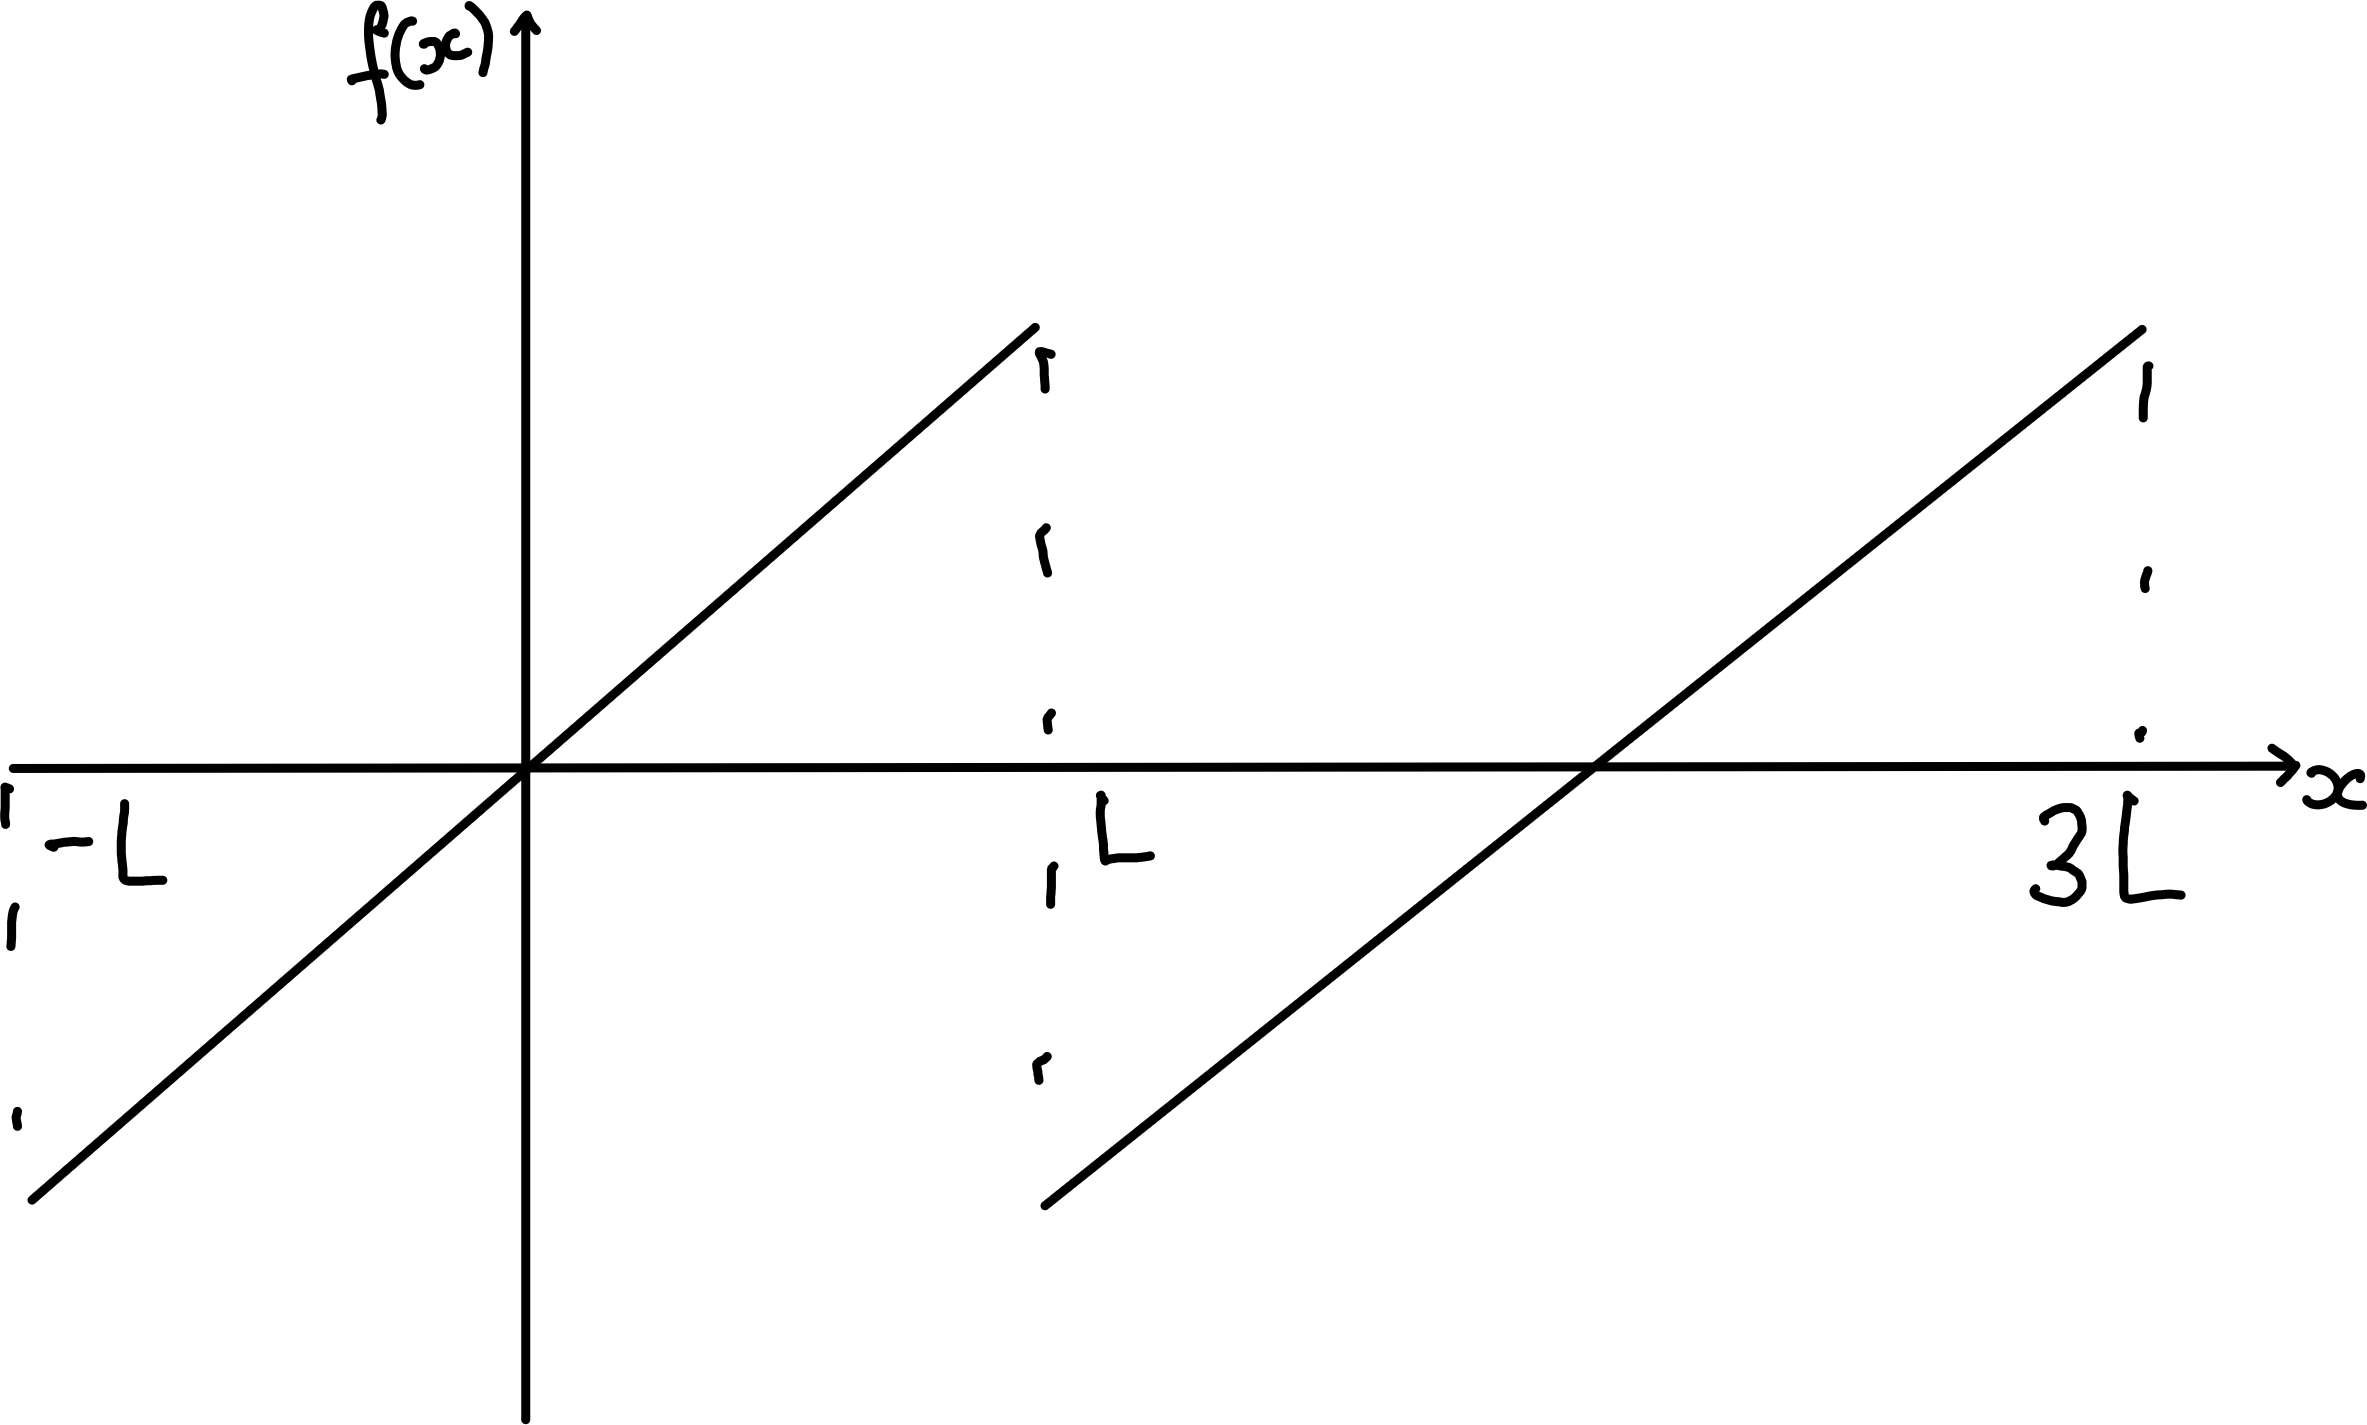
\includegraphics[height=5cm]{01-sawtooth} \par}
    Here,
    $a_n = \frac{1}{L} \int_{-L}^L x \cos \frac{n\pi x}{L} \dd{x} = 0$ as $x$ odd and $cos$ is even.
    \begin{align*}
        b_n &= \frac{1}{L} \int_{-L}^L x \sin \frac{n\pi x}{L} \dd{x} \\
        &= \frac{2}{L} \int_0^L x \sin \frac{n\pi x}{L} \dd{x} \text{ as the function we are integrating is even} \\
        &= \frac{-2}{n\pi} \qty[x \cos \frac{n\pi x}{L}]_0^L + \frac{2}{n\pi} \int_0^L \cos \frac{n \pi x}{L} \dd{x} \\
        &= \frac{-2L}{n\pi} \cos n \pi + \frac{2L}{(n\pi)^2} \sin n \pi \\
        &= \frac{2L}{n\pi} (-1)^{n+1}
    \end{align*}
    So the sawtooth FS is
    \begin{align} \label{eq:1.6}
        f(x) &= \frac{2L}{\pi} \sum_{n=1}^{\infty} \frac{(-1)^{n+1}}{n} \sin \frac{n \pi x}{L} \\
        &= \frac{2L}{\pi} \left( \sin \frac{\pi x}{L} - \frac{1}{2} \sin \frac{2 \pi x}{L} + \frac{1}{3} \sin \frac{3 \pi x}{L} + \dots \right) \notag
    \end{align} 
    which is slowly convergent.
    {\par \centering 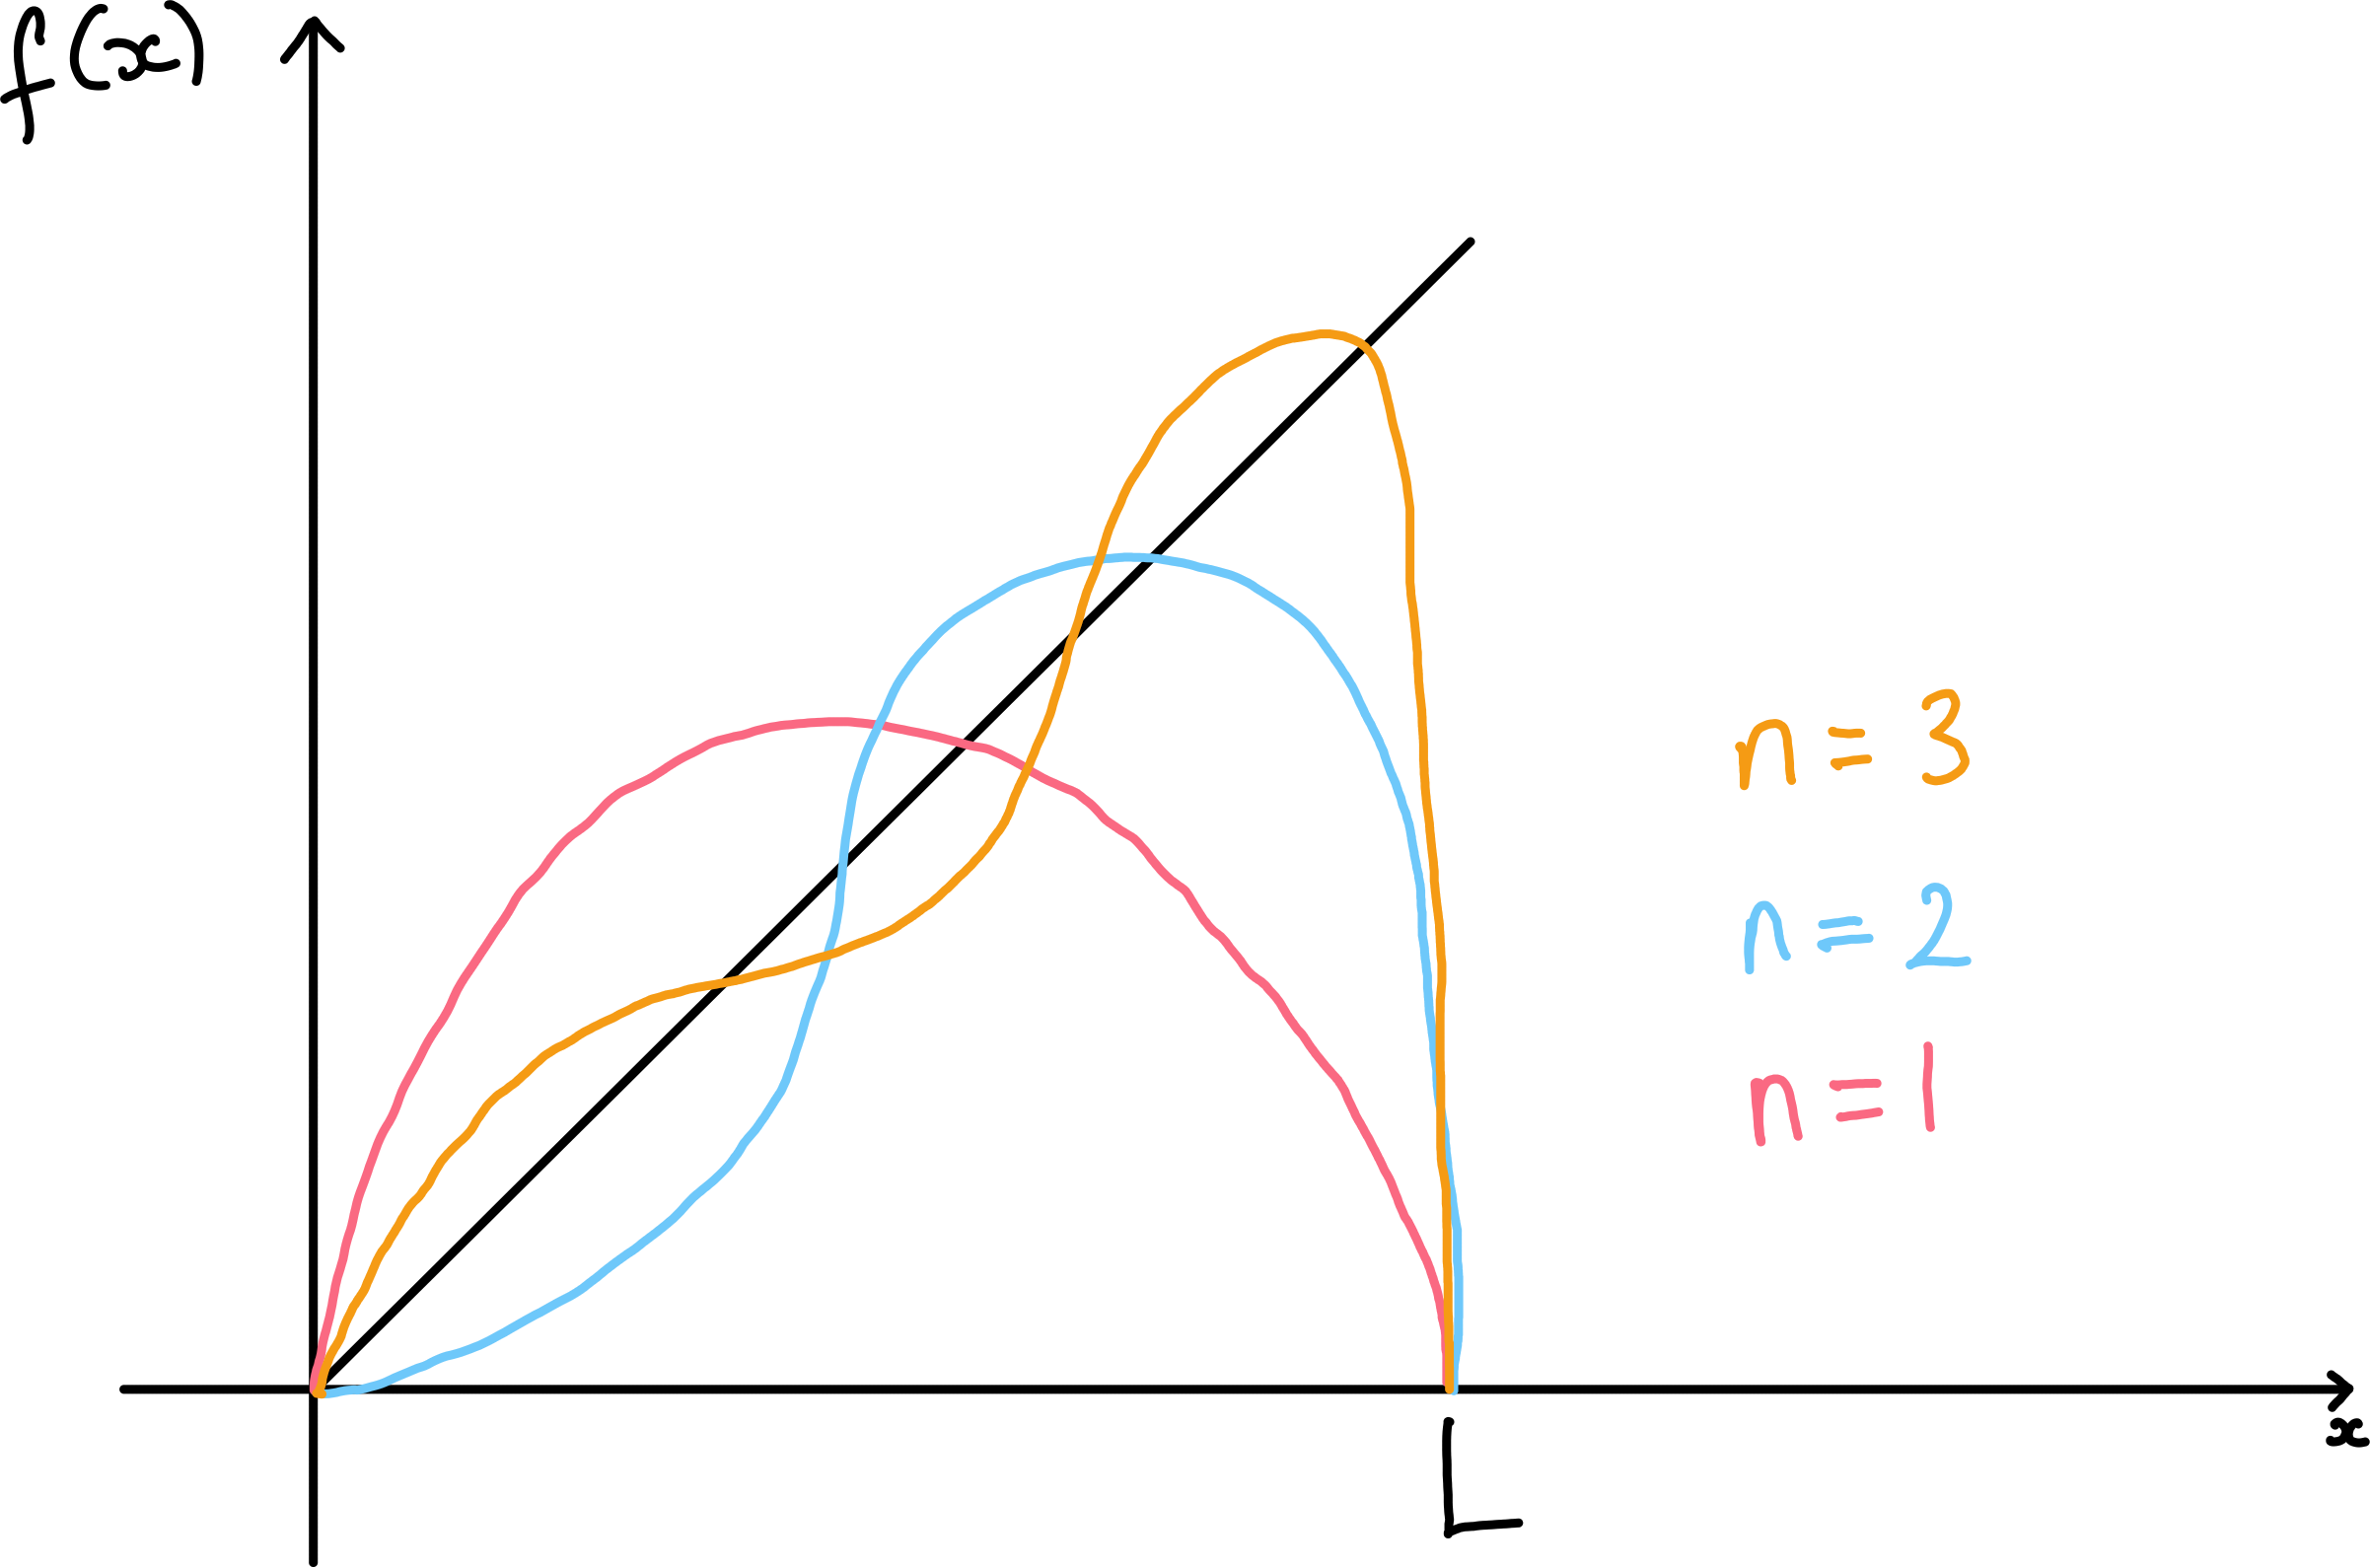
\includegraphics[height=5cm]{01-sawtooth2} \par}
\end{example}

\begin{note} As $n \to \infty$
    \begin{enumerate}
        \item FS approx improves (convergent when cts)
        \item $\text{FS} \to 0$ at $x = L$ i.e. midpoint of discontinuity
        \item FS has a persistent overshoot at $x = L$ (approx 9\% knows as Gibbs phenomenon, see Sheet 1, Q5).
    \end{enumerate} 
\end{note} 

\subsection{Dirichlet conditions}
The Dirichlet conditions are sufficiency conditions for a ``well-behaved'' function, that will imply the existence of a unique Fourier series.
\begin{theorem}
    If $f(x)$ is a bounded periodic function of period $2L$ with a finite number of minima, maxima and discontinuities in $[0, 2L)$, then the Fourier series converges to $f$ at all points at which $f$ is continuous, and at discontinuities the series converges to the midpoint.
\end{theorem}
\begin{note} \
    \begin{enumerate}
        \item These are some relatively weak conditions for convergence, compared to Taylor series.
            However, this definition still eliminates pathological functions such as $\frac{1}{x}$, $\sin \frac{1}{x}$, $\mathbbm 1 (\mathbb Q)$ and so on.
        \item \color{red}The converse is not true\color{black}; for example, $\sin \frac{1}{x}$ does in fact have a Fourier series.
        \item The proof is difficult and will not be given.
    \end{enumerate}
\end{note}

\noindent The rate of convergence of the Fourier series depends on the smoothness of the function.
\begin{theorem}
    If $f(x)$ has continuous derivatives up to a $p$th derivative which is discontinuous, then the Fourier series converges with order $O(n^{-(p+1)})$ as $n \to \infty$.
\end{theorem}
\begin{example}[$p = 0$]
    Consider the square wave (Sheet 1, Q5)
    \begin{align*}
        f(x) = \begin{cases}
            1  & 0 \leq x < 1  \\
            -1 & -1 \leq x < 0
        \end{cases}
    \end{align*}
    {\par \centering 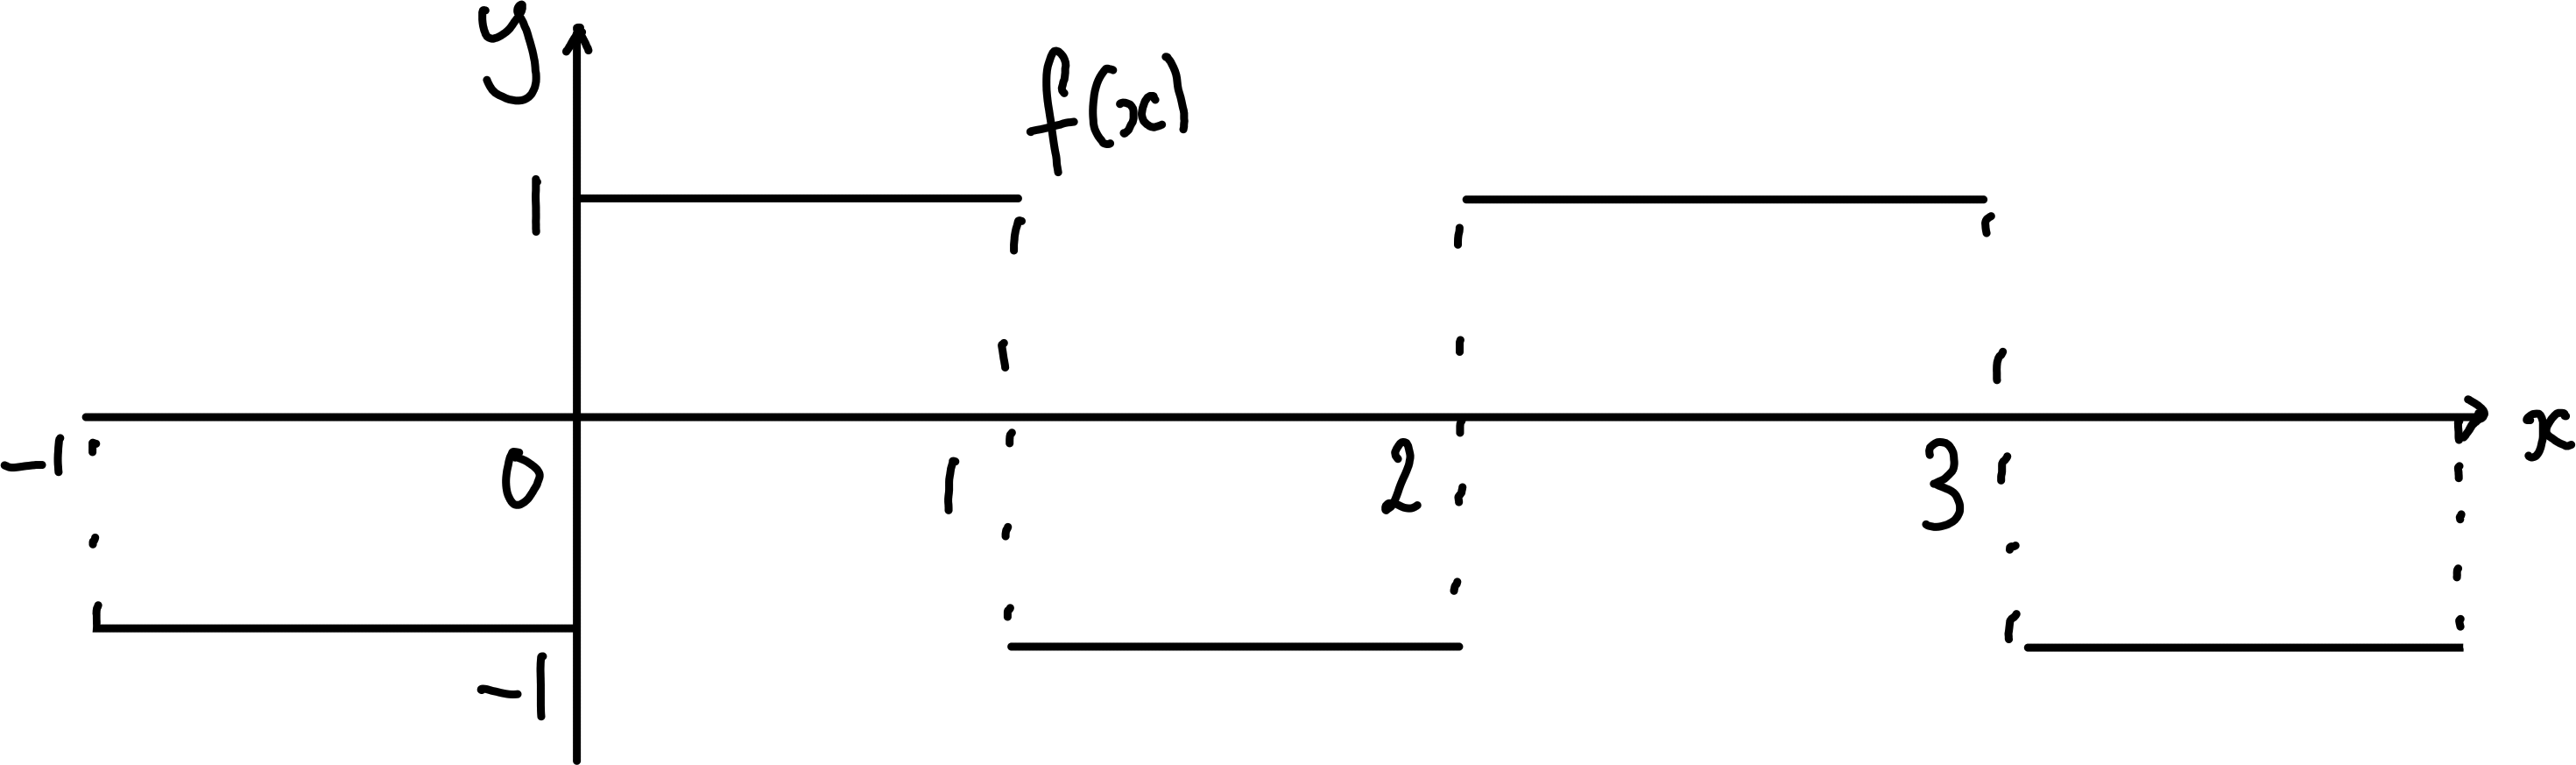
\includegraphics[height=5cm]{01-squarewave} \par}
    Then the Fourier series is
    \begin{align} \label{eq:1.7}
        f(x) = 4 \sum_{m=1}^\infty \frac{\sin (2m-1)\pi x}{(2m-1)\pi}
    \end{align}
\end{example}

\begin{example}[$p = 1$]
    Consider the general `see-saw' wave, defined by
    \begin{align*}
        f(x) = \begin{cases}
            x(1 - \xi) & 0 \leq x < \xi \\
            \xi(1 - x) & \xi \leq x < 1
        \end{cases}
    \end{align*}
    and defined as an odd function for $-1 \leq x < 0$.
    The Fourier series is\footnote{This is an important exercise you should do at home.}
    \begin{align} \label{eq:1.8}
        f(x) = 2 \sum_{m=1}^\infty \frac{\sin n\pi \xi \sin n\pi x}{(n \pi)^2}
    \end{align}
    
    {\par \centering 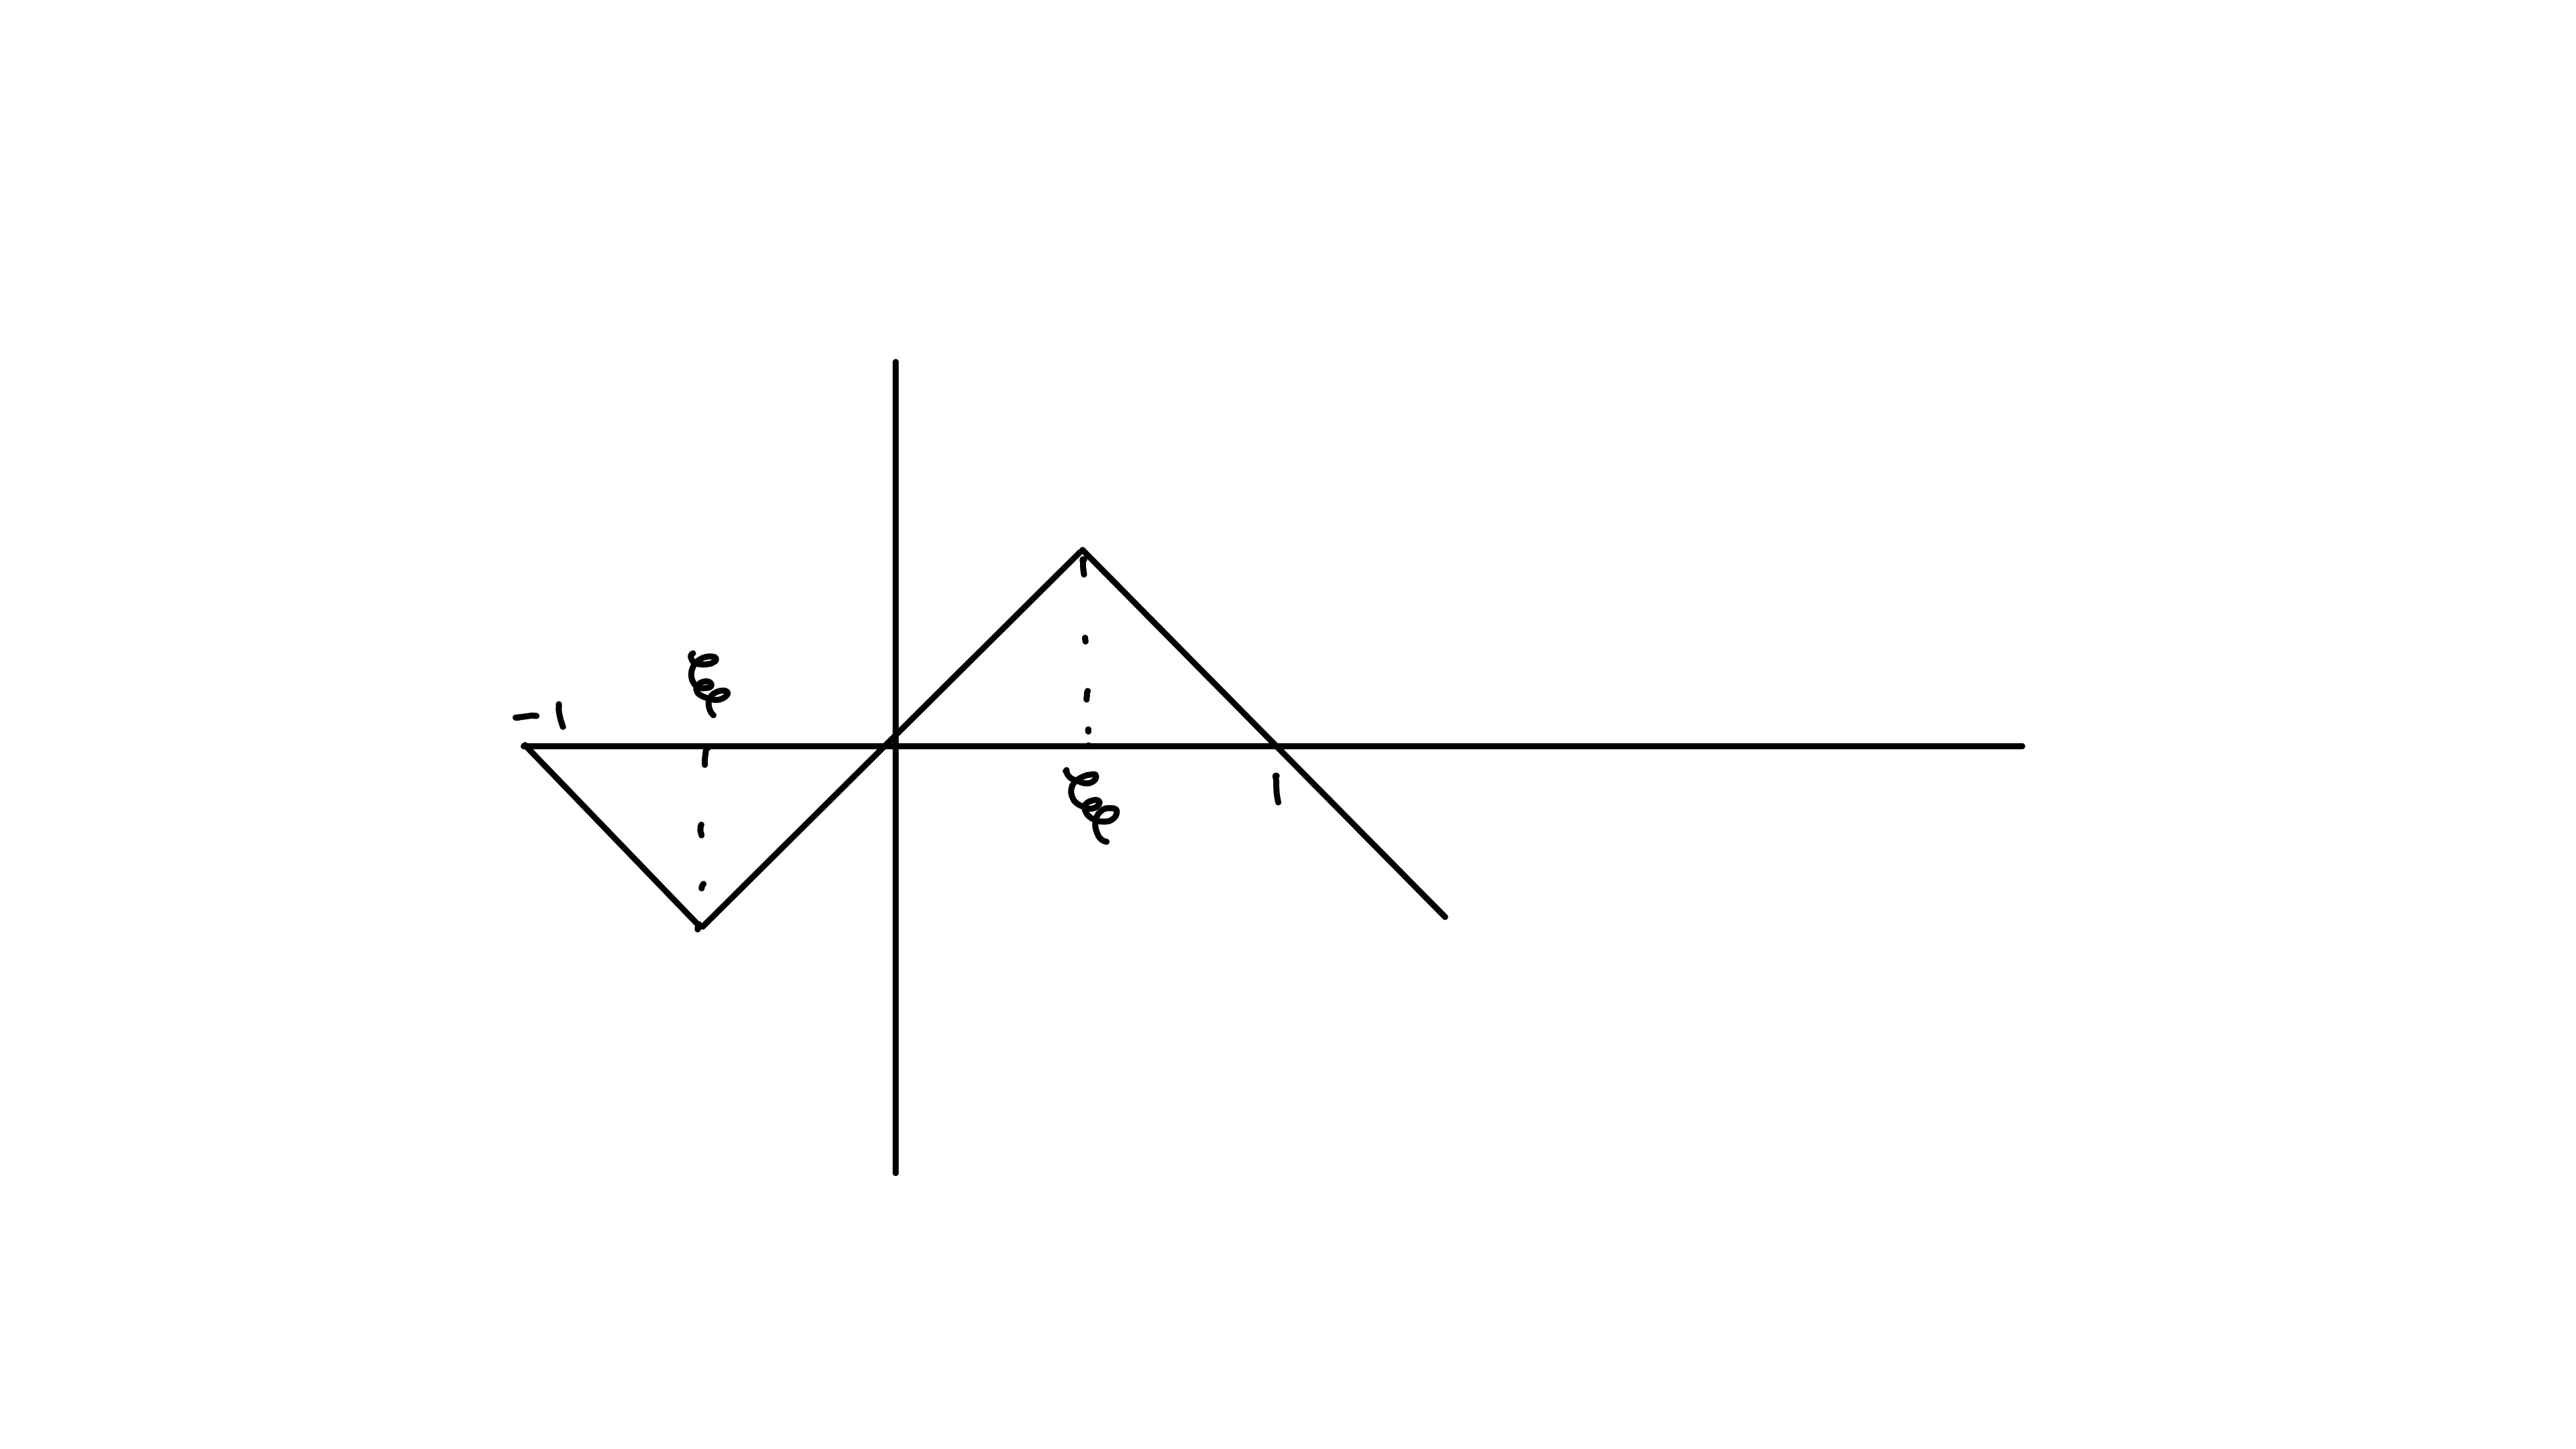
\includegraphics[height=5cm]{01-seesaw} \par}

    For instance, if $\xi = \frac{1}{2}$, we can show that
    \begin{align*}
        f(x) = 2 \sum_{m=1}^\infty (-1)^{m+1} \frac{\sin (2m-1)\pi x}{((2m-1)\pi)^2}
    \end{align*}
\end{example}
\begin{example}[$p = 2$]
    Let
    \begin{align*}
        f(x) = \frac{1}{2} x(1-x)
    \end{align*}
    for $0 \leq x < 1$, and defined as an odd function for $-1 \leq x < 0$.
    We can show that
    \begin{align} \label{eq:1.9}
        f(x) = 4\sum_{n=1}^\infty \frac{\sin(2m - 1)\pi x}{((2m-1)\pi)^3}
    \end{align}
    {\par \centering 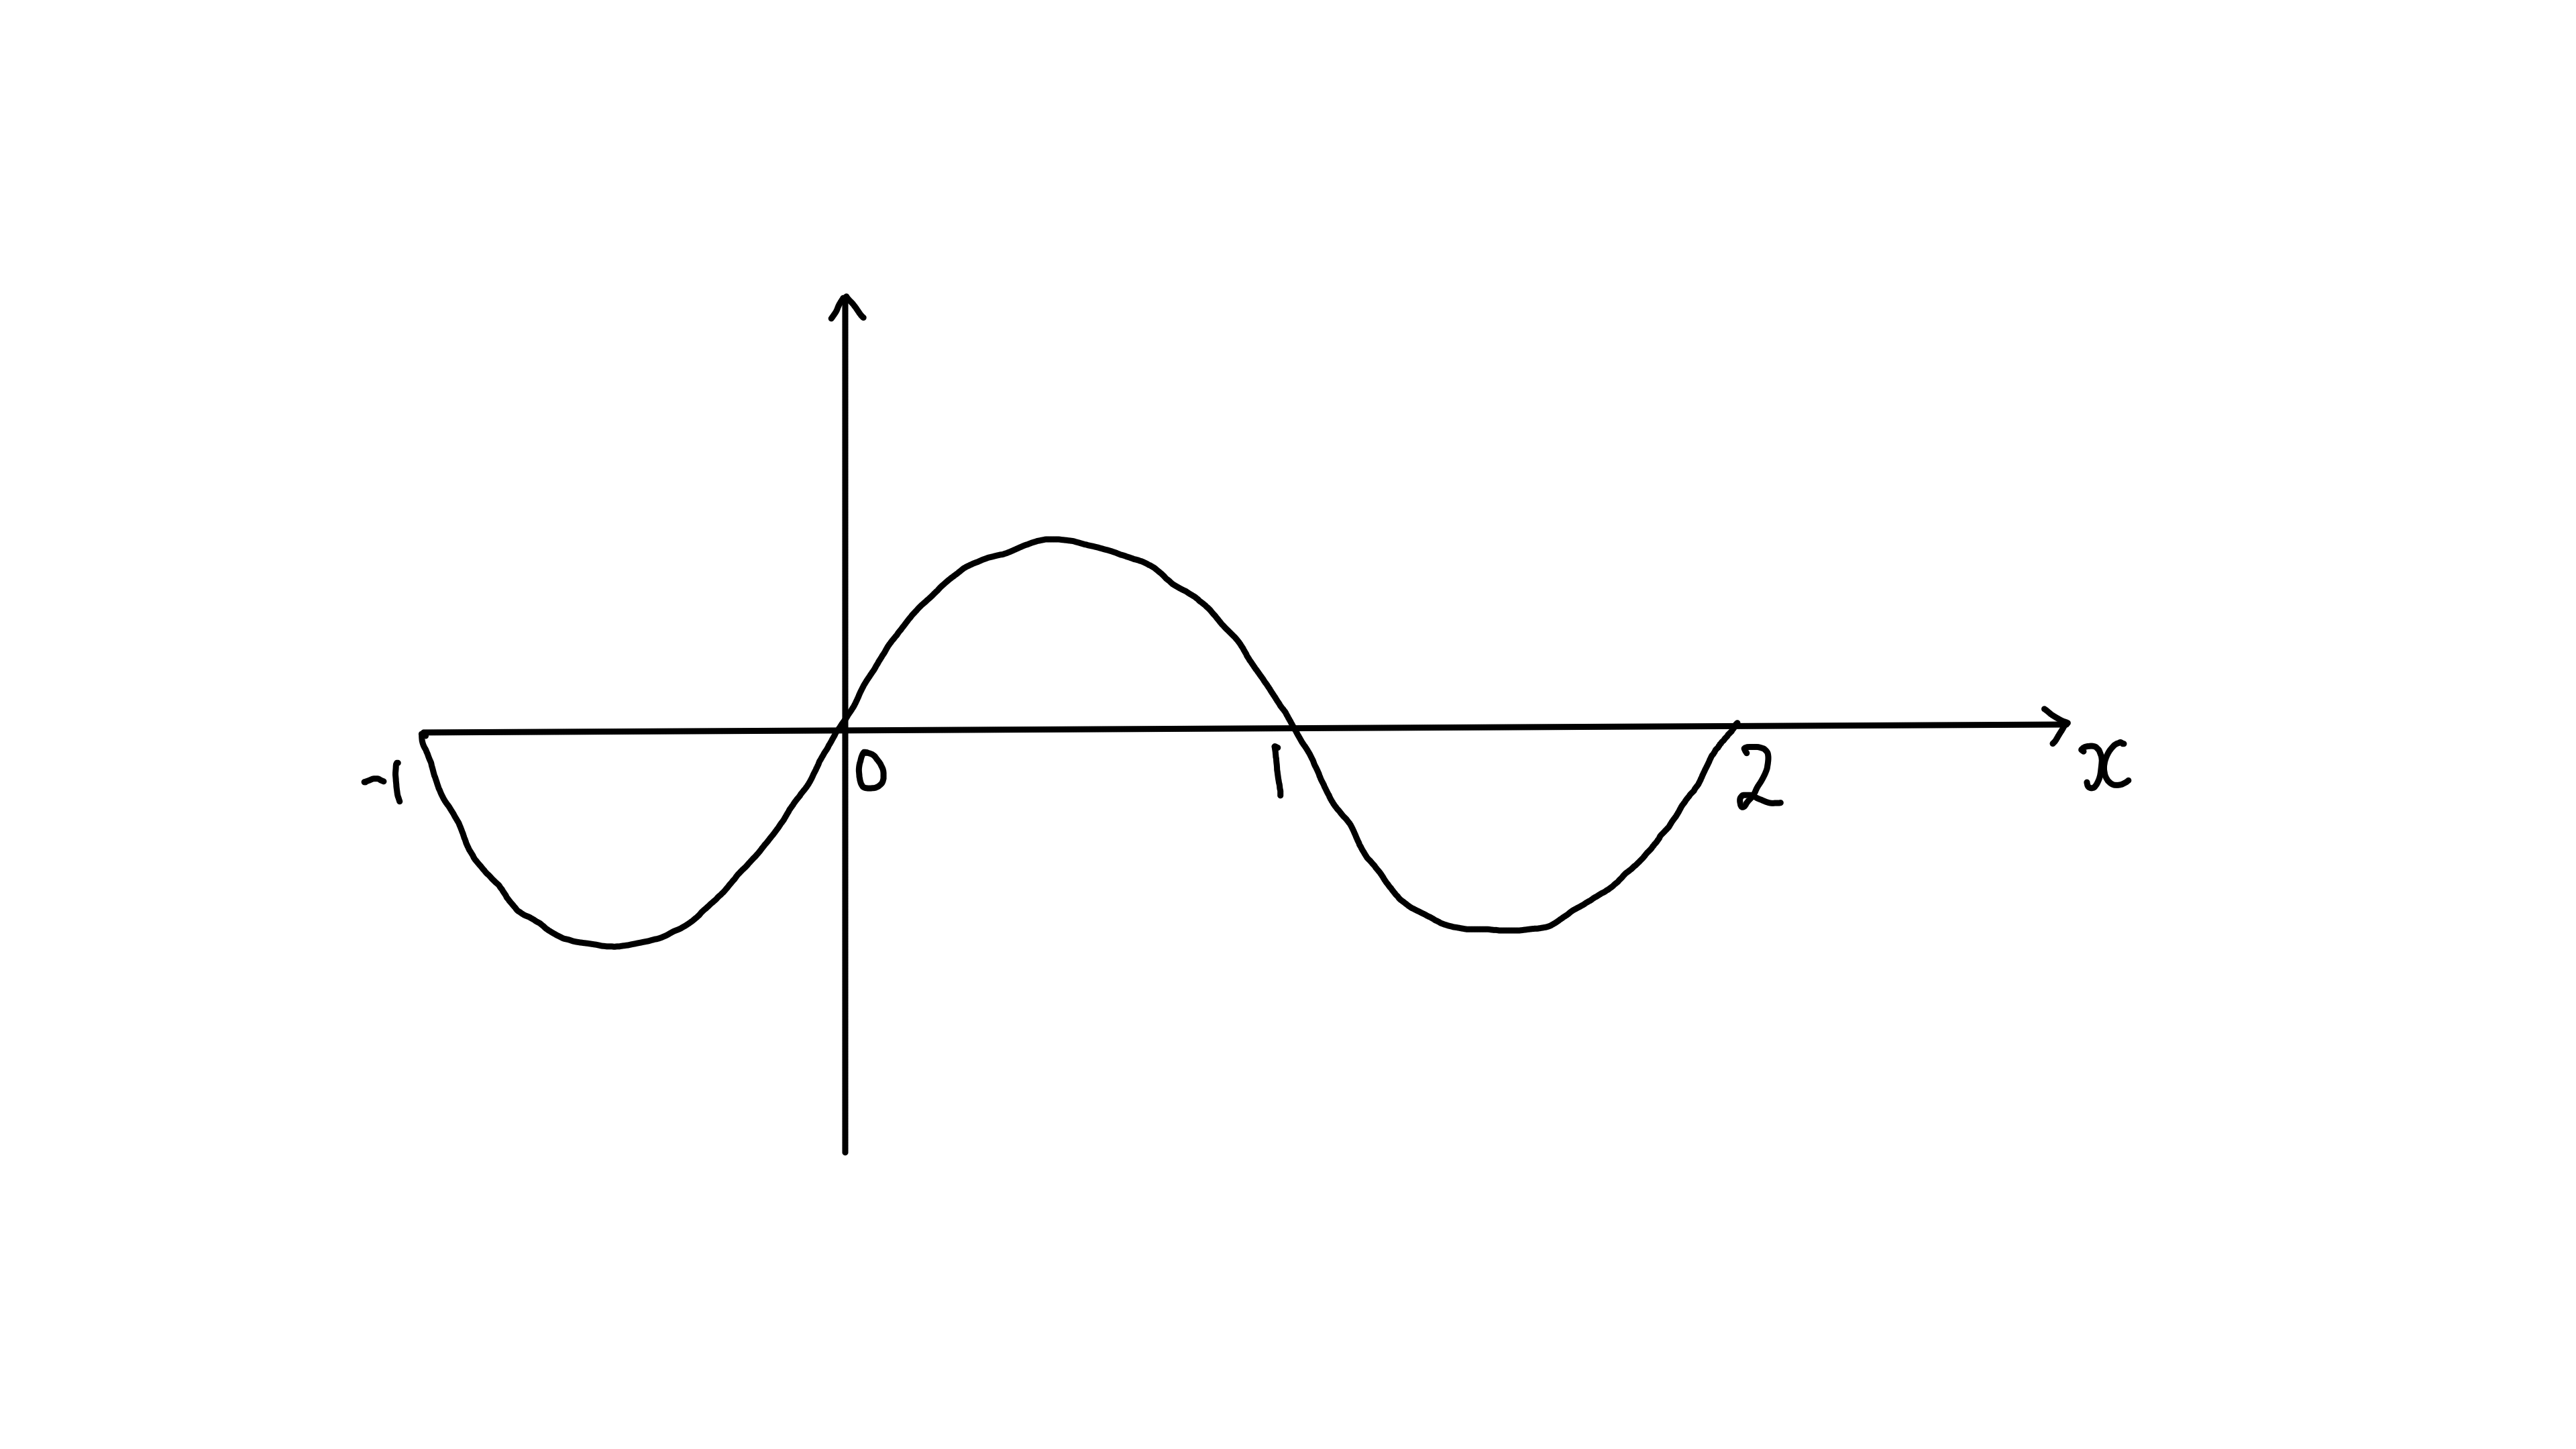
\includegraphics[height=5cm]{01-p2} \par}
\end{example}
\begin{example}[$p = 3$]
    Consider\footnote{Sheet 1, Q1}
    \begin{align*}
        f(x) = (1-x^2)^2
    \end{align*}
    with Fourier series
    \begin{align*}
        a_n = O\qty(\frac{1}{n^4})
    \end{align*}
\end{example}

\subsection{Integration of FS}
It is always valid to take the integral of a Fourier series term by term.
Defining $F(x) = \int_{-L}^x f(x) \dd{x}$, we can show that $F$ satisfies the Dirichlet conditions if $f$ does.
For instance, a jump discontinuity becomes continuous in the integral.

\subsection{Differentiation}
Differentiating term by term is not always valid.
For example, consider the square wave above:
\begin{align*}
    f(x) \stackrel{?}{=} 4 \sum_{m=1}^\infty \cos (2m-1)\pi x
\end{align*}
which is an unbounded series (consider $x = 0$).
\begin{theorem}
    If $f(x)$ is continuous and satisfies the Dirichlet conditions, and $f'(x)$ also satisfies the Dirichlet conditions, then $f'(x)$ can be found term by term by differentiating the Fourier series of $f(x)$.
\end{theorem}
\begin{example}
    We can differentiate the see-saw function, \cref{eq:1.8}, with $\xi = \frac{1}{2}$, even though the derivative is not continuous.
    The result is an offset square wave, or by mapping $x \mapsto x + \frac{1}{2}$ we recover the original square wave, \cref{eq:1.7}.
\end{example}

\subsection{Parseval's theorem}
Parseval's theorem relates the integral of the square of a function with the sum of the squares of the function's Fourier series coefficients.
\begin{theorem}[Parseval's theorem]
    Suppose $f$ has Fourier coefficients $a_i, b_i$.
    Then
    \begin{align}
        \int_0^{2L} [f(x)]^2 \dd{x} & = \int_0^{2L} \qty[ \frac{1}{2}a_0 + \sum_{n=1}^\infty a_n \cos \frac{n \pi x}{L} + \sum_{n=1}^\infty b_n \sin \frac{n\pi x}{L} ]^2 \dd{x} \notag \\
        \intertext{We can remove cross terms, since the basis functions are orthogonal. \cref{eq:1.1,eq:1.2,eq:1.3}}
        & = \int_0^{2L} \qty[ \frac{1}{4} a_0^2 + \sum_{n=1}^\infty a_n^2 \cos^2 \frac{n\pi x}{L} + \sum_{n=1}^\infty b_n^2 \sin^2 \frac{n\pi x}{L} ] \dd{x} \notag \\
        & = L \qty[ \frac{1}{2} a_0^2 + \sum_{n=1}^\infty (a_n^2 + b_n^2) ] \label{eq:1.10}
    \end{align}
\end{theorem}
\noindent This is also called the \textit{completeness relation}: the left hand side is greater than or equal to the right hand side if any of the basis functions are missing.
\begin{example}
    Let us apply Parseval's theorem to the sawtooth wave with FS \cref{eq:1.6}.
    \begin{align*}
        \int_{-L}^L [f(x)]^2 \dd{x} = \int_{-L}^L x^2 \dd{x} = \frac{2}{3}L^3
    \end{align*}
    The right hand side gives
    \begin{align*}
        L \sum_{n=1}^\infty \frac{4L^2}{n^2 \pi^2} = \frac{4 L^3}{\pi^2} \sum_{n=1}^\infty \frac{1}{n^2}
    \end{align*}
    Parseval's theorem then implies\footnote{Sheet 1, Q3}
    \begin{align*}
        \sum_{n=1}^\infty \frac{1}{n^2} = \frac{\pi^2}{6}
    \end{align*}
\end{example}
\begin{note}
    Parseval's theorem for functions $\inner{f, f} = \norm{f}^2$ is equivalent to Pythagoras for vectors $\inner{v, v} = \norm{v}^2$.
\end{note} 

\subsection{Half-range series}
Consider $f(x)$ defined only on $0 \leq x < L$.
We can extend the range of $f$ to be the full range $-L \leq x < L$ in two simple ways:
\begin{enumerate}
    \item require $f$ to be odd, so $f(-x) = -f(x)$.
        Hence, $a_n = 0$ (as $\cos$ is even) and
        \begin{align} \label{eq:1.11}
            b_n = \frac{2}{L} \int_0^L f(x) \sin \frac{n \pi x}{L} \dd{x}
        \end{align}
        So
        \begin{align*}
            f(x) = \sum_{n=1}^\infty b_n \sin \frac{n\pi x}{L}
        \end{align*}
        which is called a Fourier sine series.
    \item require $f$ to be even, so $f(-x) = f(x)$.
        In this case, $b_n = 0$ and
        \begin{align} \label{eq:1.12}
            a_n = \frac{2}{L} \int_0^L f(x) \cos \frac{n \pi x}{L} \dd{x}
        \end{align}
        and so
        \begin{align*}
            f(x) = \frac{1}{2}a_0 + \sum_{n=1}^\infty a_n \cos \frac{n\pi x}{L}
        \end{align*}
        which is a Fourier cosine series.
\end{enumerate}

\subsection{Complex representation of Fourier series}
Recall that
\begin{align*}
    \cos \frac{n \pi x}{L} &= \frac{1}{2}\qty(e^{i n \pi x / L} + e^{-i n \pi x / L}); \\
    \sin \frac{n \pi x}{L} &= \frac{1}{2i}\qty(e^{i n \pi x / L} - e^{-i n \pi x / L})
\end{align*}
Therefore, a Fourier series can be written as
\begin{align}
    f(x) &= \frac{1}{2} a_0 + \frac{1}{2} \sum_{n=1}^\infty \qty[ (a_n - i b_n) e^{i n \pi x / L} + (a_n + i b_n) e^{-i n \pi x / L} ] \notag \\
    &= \sum_{m=-\infty}^\infty c_m e^{i m \pi x / L} \label{eq:1.13}
\end{align}
where for $m > 0$ we have $m=n, c_m = \frac{1}{2}(a_n - ib_n)$, and for $m < 0$ we have $n = -m, c_m = \frac{1}{2}(a_{-m} + ib_{-m})$, and where $m = 0$ we have $c_0 = \frac{1}{2} a_0$.
In particular,
\begin{align} \label{eq:1.14}
    c_m = \frac{1}{2L} \int_{-L}^L f(x) e^{-i m \pi x / L} \dd{x}
\end{align}
where the negative sign comes from the complex conjugate.
This is because, for complex-valued $f, g$, we have
\begin{definition}[Complex inner product] ~\vspace*{-1.5\baselineskip}
    \begin{align*}
        \inner{f,g} = \int_{-L}^L f^\star\footnote{$f^\star$ is the complex conjugate of $f$.} g \dd{x}
    \end{align*}
\end{definition} 
The orthogonality conditions are
\begin{align} \label{eq:1.15}
    \int_{-L}^L e^{-i m \pi x / L} e^{i n \pi x / L} \dd{x} = 2L \delta_{mn}
\end{align}
Parseval's theorem now states
\begin{align*}
    \int_{-L}^L f^\star(x) f(x) \dd{x} = \int_{-L}^L \abs{f(x)}^2 \dd{x} = 2L \sum_{m=-\infty}^\infty \abs{c_m}^2
\end{align*}

\subsection{Self-adjoint matrices}
\textit{Much of this section is a recap of IA Vectors and Matrices.}
Suppose that $u, v \in \mathbb C^N$ with inner product
\begin{align} \label{eq:1.16}
    \inner{u,v} = u^\dagger v
\end{align}
\begin{definition}[Hermitian matrix] 
    The $N \times N$ matrix $A$ is \textit{self-adjoint}, or \textit{Hermitian}, if
    \begin{align*}
        \forall u,v \in \mathbb C^N, \inner{Au, v} = \inner{u, Av} \iff A^\dagger = A
    \end{align*}
\end{definition} 
The eigenvalues $\lambda_n$ and eigenvectors $v_n$ satisfy
\begin{align} \label{eq:1.17}
    A v_n = \lambda_n v_n
\end{align}
They have the following properties:
\begin{enumerate}
    \item $\lambda_n^\star = \lambda_n$;
    \item $\lambda_n \neq \lambda_m \implies \inner{ v_n, v_m } = 0$;
    \item we can create an orthonormal basis from the eigenvectors.
\end{enumerate}
Given $b \in \mathbb C^n$, we can solve for $x$ in the general matrix equation 
\begin{align}
    Ax = b \label{eq:1.18}
\end{align}
Express $b$ in terms of the eigenvector basis:
\begin{align*}
    b = \sum_{n=1}^N b_n v_n \notag
\end{align*}
We seek a solution of the form
\begin{align*}
    x = \sum_{n=1}^N c_n v_n
\end{align*}
At this point, the $b_n$ are known and the $c_n$ are our target.
Substituting into the matrix equation \cref{eq:1.18}, orthogonality of basis vectors gives
\begin{align*}
    A \sum_{n=1}^N c_n v_n &= \sum_{n=1}^N b_n v_n \\
    \sum_{n=1}^N c_n \lambda_n v_n &= \sum_{n=1}^N b_n v_n
    \intertext{As the eigenvector basis is orthogonal we can equate coefficients}
    c_n \lambda_n &= b_n \\
    c_n &= \frac{b_n}{\lambda_n}
\end{align*}
Therefore,
\begin{align} \label{eq:1.19}
    x = \sum_{n=1}^N \frac{b_n}{\lambda_n} v_n
\end{align}
provided $\lambda_n \neq 0$, or equivalently, the matrix is invertible.

\subsection{Solving inhomogeneous ODEs with Fourier series}
We wish to find $y(x)$ given a driving/ source term $f(x)$ for the general differential equation
\begin{align} \label{eq:1.20}
    \mathcal L y \equiv -\dv[2]{y}{x} = f(x)
\end{align}
with boundary conditions $y(0) = y(L) = 0$.
The related eigenvalue problem is
\begin{align*}
    \mathcal L y_n = \lambda_n y_n,\quad y_n(0) = y_n(L) = 0
\end{align*}
which has solutions
\begin{align} \label{eq:1.21}
    y_n(x) = \sin \frac{n \pi x}{L},\ \lambda_n = \qty(\frac{n\pi}{L})^2
\end{align}
We can show that this is a self-adjoint linear operator\footnote{https://math.stackexchange.com/questions/4356100/why-is-the-second-derivative-operator-self-adjoint} with orthogonal eigenfunctions.
We seek solutions of the form of a half-range sine series.
Consider
\begin{align*}
    y(x) = \sum_{n=1}^\infty c_n \sin\frac{n \pi x}{L}
\end{align*}
The right hand side is
\begin{align*}
    f(x) = \sum_{n=1}^\infty b_n \sin \frac{n \pi x}{L}
\end{align*}
We can find $b_n$ by
\begin{align*}
    b_n = \frac{2}{L} \int_0^L f(x) \sin \frac{n \pi x}{L} \dd{x}
\end{align*}
Substituting into \cref{eq:1.20}, we have
\begin{align*}
    \mathcal L y = -\dv[2]{x} \qty(\sum_n c_n \sin \frac{n \pi x}{L}) &= \sum_n c_n \qty(\frac{n\pi}{L})^2 \sin \frac{n \pi x}{L} \\
    \text{So } \sum_n c_n \qty(\frac{n\pi}{L})^2 \sin \frac{n \pi x}{L} &= \sum_n b_n \sin \frac{n \pi x}{L}
\end{align*}
By orthogonality \cref{eq:1.1},
\begin{align*}
    c_n \qty(\frac{n \pi}{L})^2 = b_n \implies c_n = \qty(\frac{L}{n \pi})^2 b_n
\end{align*}
Therefore the solution is
\begin{align} \label{eq:1.22}
    y(x) = \sum_n \qty(\frac{L}{n \pi})^2 b_n \sin \frac{n \pi x}{L} = \sum_n \frac{b_n}{\lambda_n} y_n
\end{align}
which is equivalent to the solution we found for self-adjoint matrices for which the eigenvalues and eigenvectors are known.
\begin{example}[Odd square wave]
    Consider an odd square wave with $L = 1$, so $f(x) = 1$ from $0 \leq x < 1$.
    \begin{align*}
        f(x) = 4 \sum_m \frac{\sin(2m-1)\pi x}{(2m-1)\pi} \text{ by \cref{eq:1.7}}
    \end{align*}
    Then the solution to $\mathcal L y = f$ \cref{eq:1.22} should be (with odd $n = 2m-1$)
    \begin{align*}
        y(x) = \sum_n \frac{b_n}{\lambda_n} y_n = 4 \sum_n \frac{\sin (2m-1) \pi x}{((2m - 1) \pi)^3}
    \end{align*}
    This is exactly the Fourier series for
    \begin{align*}
        y(x) = \frac{1}{2}x(1-x) \text{ by \cref{eq:1.9}}
    \end{align*}
    so this $y$ is the solution to the differential equation.
    We can in fact integrate $\mathcal L y = 1$ directly with the boundary conditions to verify the solution.
    We can also differentiate the Fourier series for $y$ twice to find the square wave.
\end{example}